\documentclass[journal,12pt,two column]{IEEEtran}
\usepackage{setspace}
\usepackage{enumitem}
\usepackage[cmex10]{amsmath}
\usepackage{tfrupee}
\usepackage{amsthm}
\usepackage[utf8]{inputenc}
\usepackage{graphicx}
\title{ASSIGNMENT 1 }
\author{Muskan Jaiswal - cs21btech11037}
\newcommand{\solution}{\noindent \textbf{Solution: }}
\begin{document}
\maketitle
\textbf{Problem 1(b):} Solve the equation $4x^2-5x-3=0$ and give your answer correct to 2 decimal places
\bigskip

\textbf{SOLUTION:}     For any kind of equation of the form  $ax^2+bx+c=0$

It's roots are

$x=\frac{-b\pm\sqrt{b^2-4ac}}{2a}$

For the given equation-
\begin{equation}
    4x^2-5x-3=0
\end{equation}
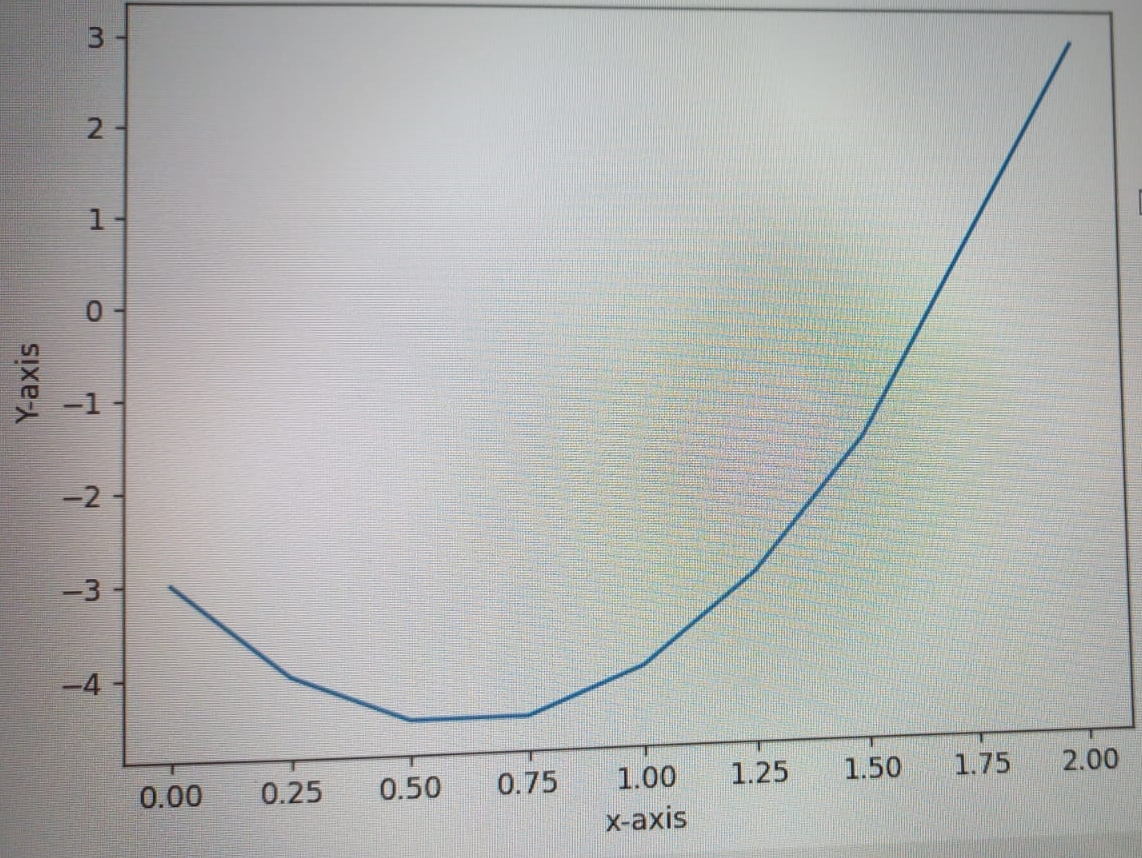
\includegraphics[width=\linewidth]{1128.jpeg}

roots upto two decimal places are
$x1=\frac{5+\sqrt{(-5)^2-4*4*(-3)}}{2*4}
$\\


$x1=\frac{5+\sqrt{25+48}}{8}
$
\\
$x1=\frac{5+\sqrt{73}}{8}
$
\\
$x1=\frac{5+8.54}{8}
$ \\

$x1=\frac{13.54}{8}
$
\\
$ x1=1.69
  $\\


and

$x2=\frac{5-\sqrt{(-5)^2-4*4*(-3)}}{2*4}
$\\

$x2=\frac{5-\sqrt{25+48}}{8}
$\\

$x2=\frac{5-\sqrt{73}}{8}
$\\

$x2=\frac{5-8.54}{8} $\\

$x2=\frac{-3.54}{8} $\\

$x2=-0.44
$
\bigskip

The roots of the given equation are 1.69 and -0.44
\end{document}













